\documentclass{beamer}
\mode<presentation>{\usecolortheme{crane}}
\usetheme{Madrid}

\usepackage{graphicx}
\usepackage[utf8]{inputenc}

\title{CS633 Project: Parallel Debugger}
\author[Milind, Subhdeep]{Milind Luthra (150363) \and Subhdeep Saha (150732)}

\date{15 March 2019}

\AtBeginSection[]
{
  \begin{frame}{Table of Contents}
    \tableofcontents[currentsection]
  \end{frame}
}

\AtBeginSubsection[]
{
  \begin{frame}{Table of Contents}
    \tableofcontents[currentsubsection]
  \end{frame}
}

\begin{document}

\frame{\titlepage}

\section{Overview}
\begin{frame}
\frametitle{Sample frame title}
This is a text in the first frame. This is a text in the first frame. This is a text in the first frame.
\end{frame}

\subsection{Related Work}

\begin{frame}
  \frametitle{Allinea DDT and Totalview}
  \begin{itemize}
  \item <1-> Debuggers already in use to debug large parallel applications.
  \item <2-> Both have a rich feature set and GUIs.
  \item <3-> However, both are proprietary, commercial software.
  \item <5-> Restrictive licenses (locked to one node, or four processes etc) and high cost (a few hundred dollars).
  \item <6-> Can't be extended any further.
  \end{itemize}
\end{frame}

\begin{frame}[fragile]
  \frametitle{Using XTerm and GDB}
  \begin{itemize}
  \item <1-> Possible Idea: For n processes, launching n XTerm instances with gdb.
  \item <2-> Each terminal can be used to debug the individual processes.
  \item <3-> \texttt{mpiexec -n 4 xterm -e gdb ./test}
  \end{itemize}
\end{frame}

\begin{frame}
  \frametitle{Problems with XTerm + GDB}
  \texttt{mpiexec -n 30 xterm -e gdb ./test}

  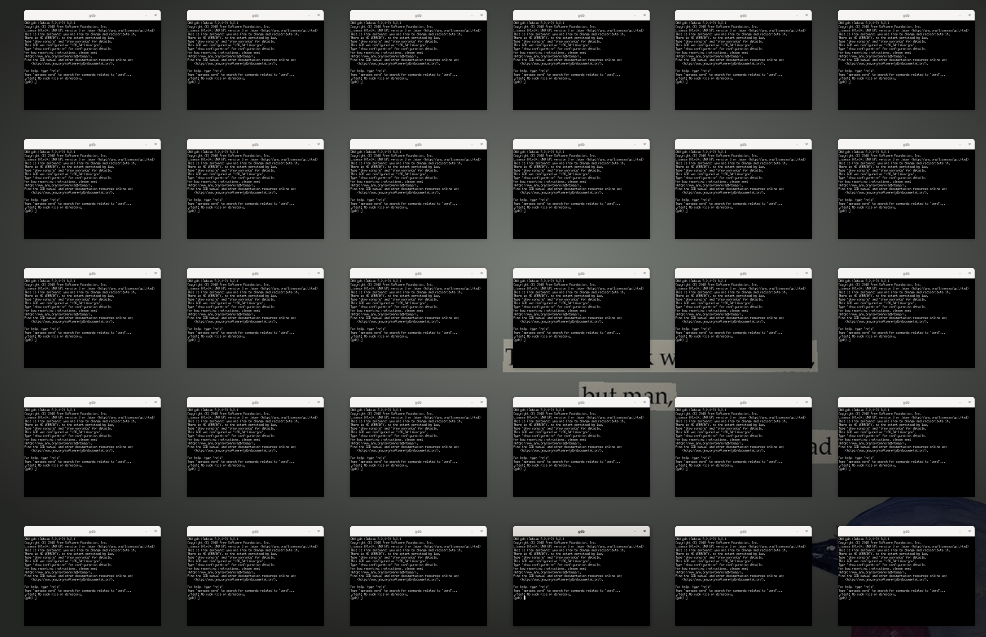
\includegraphics[width=0.9\textwidth]{usingxterm}
\end{frame}


\subsection{Idea}
\begin{frame}
  \frametitle{Basic Idea}
\begin{itemize}
  \item <1-> The basic idea is to launch a number of clients on nodes using \texttt{mpiexec}.
  \item <2-> Each client instance will run a \texttt{gdb} instance with the program to be debugged.
  \item <3-> All the instances of \texttt{gdb} are controlled using a single, centralized interface.
\end{itemize}
\end{frame}

\begin{frame}
  \frametitle{Basic Idea}
   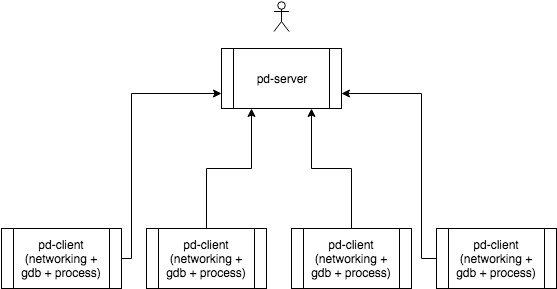
\includegraphics[width=0.8\textwidth]{flow}
\end{frame}
\section{Implementation}

\section{Features}


\end{document}